%% Beginning of file 'sample631.tex'
%%
%% Modified 2022 May  
%%
%% This is a sample manuscript marked up using the
%% AASTeX v6.31 LaTeX 2e macros.
%%
%% AASTeX is now based on Alexey Vikhlinin's emulateapj.cls 
%% (Copyright 2000-2015).  See the classfile for details.

%% AASTeX requires revtex4-1.cls and other external packages such as
%% latexsym, graphicx, amssymb, longtable, and epsf.  Note that as of 
%% Oct 2020, APS now uses revtex4.2e for its journals but remember that 
%% AASTeX v6+ still uses v4.1. All of these external packages should 
%% already be present in the modern TeX distributions but not always.
%% For example, revtex4.1 seems to be missing in the linux version of
%% TexLive 2020. One should be able to get all packages from www.ctan.org.
%% In particular, revtex v4.1 can be found at 
%% https://www.ctan.org/pkg/revtex4-1.

%% The first piece of markup in an AASTeX v6.x document is the \documentclass
%% command. LaTeX will ignore any data that comes before this command. The 
%% documentclass can take an optional argument to modify the output style.
%% The command below calls the preprint style which will produce a tightly 
%% typeset, one-column, single-spaced document.  It is the default and thus
%% does not need to be explicitly stated.
%%
%% using aastex version 6.3
\documentclass[twocolumn]{aastex631}

%% The default is a single spaced, 10 point font, single spaced article.
%% There are 5 other style options available via an optional argument. They
%% can be invoked like this:
%%
%% \documentclass[arguments]{aastex631}
%% 
%% where the layout options are:
%%
%%  twocolumn   : two text columns, 10 point font, single spaced article.
%%                This is the most compact and represent the final published
%%                derived PDF copy of the accepted manuscript from the publisher
%%  manuscript  : one text column, 12 point font, double spaced article.
%%  preprint    : one text column, 12 point font, single spaced article.  
%%  preprint2   : two text columns, 12 point font, single spaced article.
%%  modern      : a stylish, single text column, 12 point font, article with
%% 		  wider left and right margins. This uses the Daniel
%% 		  Foreman-Mackey and David Hogg design.
%%  RNAAS       : Supresses an abstract. Originally for RNAAS manuscripts 
%%                but now that abstracts are required this is obsolete for
%%                AAS Journals. Authors might need it for other reasons. DO NOT
%%                use \begin{abstract} and \end{abstract} with this style.
%%
%% Note that you can submit to the AAS Journals in any of these 6 styles.
%%
%% There are other optional arguments one can invoke to allow other stylistic
%% actions. The available options are:
%%
%%   astrosymb    : Loads Astrosymb font and define \astrocommands. 
%%   tighten      : Makes baselineskip slightly smaller, only works with 
%%                  the twocolumn substyle.
%%   times        : uses times font instead of the default
%%   linenumbers  : turn on lineno package.
%%   trackchanges : required to see the revision mark up and print its output
%%   longauthor   : Do not use the more compressed footnote style (default) for 
%%                  the author/collaboration/affiliations. Instead print all
%%                  affiliation information after each name. Creates a much 
%%                  longer author list but may be desirable for short 
%%                  author papers.
%% twocolappendix : make 2 column appendix.
%%   anonymous    : Do not show the authors, affiliations and acknowledgments 
%%                  for dual anonymous review.
%%
%% these can be used in any combination, e.g.
%%
%% \documentclass[twocolumn,linenumbers,trackchanges]{aastex631}
%%
%% AASTeX v6.* now includes \hyperref support. While we have built in specific
%% defaults into the classfile you can manually override them with the
%% \hypersetup command. For example,
%%
%% \hypersetup{linkcolor=red,citecolor=green,filecolor=cyan,urlcolor=magenta}
%%
%% will change the color of the internal links to red, the links to the
%% bibliography to green, the file links to cyan, and the external links to
%% magenta. Additional information on \hyperref options can be found here:
%% https://www.tug.org/applications/hyperref/manual.html#x1-40003
%%
%% Note that in v6.3 "bookmarks" has been changed to "true" in hyperref
%% to improve the accessibility of the compiled pdf file.
%%
%% If you want to create your own macros, you can do so
%% using \newcommand. Your macros should appear before
%% the \begin{document} command.
%%
\newcommand{\vdag}{(v)^\dagger}
\newcommand\aastex{AAS\TeX}
\newcommand\latex{La\TeX}

%% Reintroduced the \received and \accepted commands from AASTeX v5.2
%\received{March 1, 2021}
%\revised{April 1, 2021}
%\accepted{\today}

%% Command to document which AAS Journal the manuscript was submitted to.
%% Adds "Submitted to " the argument.
%\submitjournal{PSJ}

%% For manuscript that include authors in collaborations, AASTeX v6.31
%% builds on the \collaboration command to allow greater freedom to 
%% keep the traditional author+affiliation information but only show
%% subsets. The \collaboration command now must appear AFTER the group
%% of authors in the collaboration and it takes TWO arguments. The last
%% is still the collaboration identifier. The text given in this
%% argument is what will be shown in the manuscript. The first argument
%% is the number of author above the \collaboration command to show with
%% the collaboration text. If there are authors that are not part of any
%% collaboration the \nocollaboration command is used. This command takes
%% one argument which is also the number of authors above to show. A
%% dashed line is shown to indicate no collaboration. This example manuscript
%% shows how these commands work to display specific set of authors 
%% on the front page.
%%
%% For manuscript without any need to use \collaboration the 
%% \AuthorCollaborationLimit command from v6.2 can still be used to 
%% show a subset of authors.
%
%\AuthorCollaborationLimit=2
%
%% will only show Schwarz & Muench on the front page of the manuscript
%% (assuming the \collaboration and \nocollaboration commands are
%% commented out).
%%
%% Note that all of the author will be shown in the published article.
%% This feature is meant to be used prior to acceptance to make the
%% front end of a long author article more manageable. Please do not use
%% this functionality for manuscripts with less than 20 authors. Conversely,
%% please do use this when the number of authors exceeds 40.
%%
%% Use \allauthors at the manuscript end to show the full author list.
%% This command should only be used with \AuthorCollaborationLimit is used.

%% The following command can be used to set the latex table counters.  It
%% is needed in this document because it uses a mix of latex tabular and
%% AASTeX deluxetables.  In general it should not be needed.
%\setcounter{table}{1}

%%%%%%%%%%%%%%%%%%%%%%%%%%%%%%%%%%%%%%%%%%%%%%%%%%%%%%%%%%%%%%%%%%%%%%%%%%%%%%%%
%%
%% The following section outlines numerous optional output that
%% can be displayed in the front matter or as running meta-data.
%%
%% If you wish, you may supply running head information, although
%% this information may be modified by the editorial offices.
%\shorttitle{AASTeX v6.3.1 Sample article}
%\shortauthors{Schwarz et al.}
%%
%% You can add a light gray and diagonal water-mark to the first page 
%% with this command:
%% \watermark{text}
%% where "text", e.g. DRAFT, is the text to appear.  If the text is 
%% long you can control the water-mark size with:
%% \setwatermarkfontsize{dimension}
%% where dimension is any recognized LaTeX dimension, e.g. pt, in, etc.
%%
%%%%%%%%%%%%%%%%%%%%%%%%%%%%%%%%%%%%%%%%%%%%%%%%%%%%%%%%%%%%%%%%%%%%%%%%%%%%%%%%
%\graphicspath{{./}{figures/}}
%% This is the end of the preamble.  Indicate the beginning of the
%% manuscript itself with \begin{document}.

\begin{document}

%what is the average specific angular momentum? Is it the same or different than
%the halos of either galaxy before they merged

\title{Average Specific Angular Momentum of Haloes of Milky Way, M31,\\ and their Merger Remnant}

%% LaTeX will automatically break titles if they run longer than
%% one line. However, you may use \\ to force a line break if
%% you desire. In v6.31 you can include a footnote in the title.

%% A significant change from earlier AASTEX versions is in the structure for 
%% calling author and affiliations. The change was necessary to implement 
%% auto-indexing of affiliations which prior was a manual process that could 
%% easily be tedious in large author manuscripts.
%%
%% The \author command is the same as before except it now takes an optional
%% argument which is the 16 digit ORCID. The syntax is:
%% \author[xxxx-xxxx-xxxx-xxxx]{Author Name}
%%
%% This will hyperlink the author name to the author's ORCID page. Note that
%% during compilation, LaTeX will do some limited checking of the format of
%% the ID to make sure it is valid. If the "orcid-ID.png" image file is 
%% present or in the LaTeX pathway, the OrcID icon will appear next to
%% the authors name.
%%
%% Use \affiliation for affiliation information. The old \affil is now aliased
%% to \affiliation. AASTeX v6.31 will automatically index these in the header.
%% When a duplicate is found its index will be the same as its previous entry.
%%
%% Note that \altaffilmark and \altaffiltext have been removed and thus 
%% can not be used to document secondary affiliations. If they are used latex
%% will issue a specific error message and quit. Please use multiple 
%% \affiliation calls for to document more than one affiliation.
%%
%% The new \altaffiliation can be used to indicate some secondary information
%% such as fellowships. This command produces a non-numeric footnote that is
%% set away from the numeric \affiliation footnotes.  NOTE that if an
%% \altaffiliation command is used it must come BEFORE the \affiliation call,
%% right after the \author command, in order to place the footnotes in
%% the proper location.
%%
%% Use \email to set provide email addresses. Each \email will appear on its
%% own line so you can put multiple email address in one \email call. A new
%% \correspondingauthor command is available in V6.31 to identify the
%% corresponding author of the manuscript. It is the author's responsibility
%% to make sure this name is also in the author list.
%%
%% While authors can be grouped inside the same \author and \affiliation
%% commands it is better to have a single author for each. This allows for
%% one to exploit all the new benefits and should make book-keeping easier.
%%
%% If done correctly the peer review system will be able to
%% automatically put the author and affiliation information from the manuscript
%% and save the corresponding author the trouble of entering it by hand.

%\correspondingauthor{August Muench}
%\email{greg.schwarz@aas.org, gus.muench@aas.org}

\author[0000-0003-4508-2436]{Ritvik Basant}
\affiliation{Steward Observatory and Department of Astronomy, The University of Arizona, Tucson, AZ 85721, USA}

%% Note that the \and command from previous versions of AASTeX is now
%% depreciated in this version as it is no longer necessary. AASTeX 
%% automatically takes care of all commas and "and"s between authors names.

%% AASTeX 6.31 has the new \collaboration and \nocollaboration commands to
%% provide the collaboration status of a group of authors. These commands 
%% can be used either before or after the list of corresponding authors. The
%% argument for \collaboration is the collaboration identifier. Authors are
%% encouraged to surround collaboration identifiers with ()s. The 
%% \nocollaboration command takes no argument and exists to indicate that
%% the nearby authors are not part of surrounding collaborations.

%% Mark off the abstract in the ``abstract'' environment. 


%% Keywords should appear after the \end{abstract} command. 
%% The AAS Journals now uses Unified Astronomy Thesaurus concepts:
%% https://astrothesaurus.org
%% You will be asked to selected these concepts during the submission process
%% but this old "keyword" functionality is maintained in case authors want
%% to include these concepts in their preprints.
\keywords{}

%% From the front matter, we move on to the body of the paper.
%% Sections are demarcated by \section and \subsection, respectively.
%% Observe the use of the LaTeX \label
%% command after the \subsection to give a symbolic KEY to the
%% subsection for cross-referencing in a \ref command.
%% You can use LaTeX's \ref and \label commands to keep track of
%% cross-references to sections, equations, tables, and figures.
%% That way, if you change the order of any elements, LaTeX will
%% automatically renumber them.
%%
%% We recommend that authors also use the natbib \citep
%% and \citet commands to identify citations.  The citations are
%% tied to the reference list via symbolic KEYs. The KEY corresponds
%% to the KEY in the \bibitem in the reference list below. 

\section{Introduction} \label{sec:intro}

\subsection{Discussion of General Physical Background and Definition of the Topic}

The first evidence of Dark Matter (DM) came with Zwicky's analysis of fast-moving galaxies in the Coma Cluster \citep{1933AcHPh...6..110Z}. Later, while analyzing the rotation curve of the Andromeda galaxy, Vera Rubin provided yet another evidence for the existence of DM haloes surrounding galaxies \citep{1970ApJ...159..379R}. In the following years, several extensive studies were carried out and DM haloes were identified as the breeding grounds for galaxies \citep[see e.g.,][]{1978MNRAS.183..341W}. Since then, the scientific community has aimed to better constrain the properties of the DM haloes \citep[see e.g.,][analyze the triaxial shape of DM haloes]{1985ApJ...292..371D}. This paper focuses on another specific property of these DM haloes- their Average Specific Angular Momentum (ASAM), i.e., their average spin. We aim to study the ASAM of haloes surrounding the Milky Way galaxy, the M31 galaxy, and their merger remnant. 

\subsection{Overview of Current Understanding of the Halo Spin}

With the help of numerical simulations, it had been established very early that the haloes tend to rotate \citep{1987ApJ...319..575B}. Though more massive haloes appear to spin slowly, the exact strength of the spin and the halo mass depends on the definition of the halo \citep{2007MNRAS.376..215B}. The internal distribution of specific angular momentum inside a halo follows a rather simple trend -- it increases with the distance from the center \citep{2012AnP...524..507F}. The alignment of the spin axis of haloes with their three principal axes assumes a broad distribution \citep[see e.g., ][]{2006ApJ...646..815S, 2007MNRAS.376..215B}. Moreover, the direction of the angular momentum inside the halo also varies with the distance from the center \citep{2010MNRAS.404.1137B}. 

\citet{2019MNRAS.487..993D} analyzed the merger remnant of two equal-massed haloes (without baryons) with various density profiles. The authors find that the remnant halo may assume a complicated spin. Figure~\ref{Paper} shows how the spin of the remnant halo varies with the dimensionless energy parameter (K; tells the energy of the colliding haloes) analyzed in \citet{2019MNRAS.487..993D}. \citet{2010MNRAS.407..435A} examine the effects of the formation of a central galaxy on its surrounding halo. When the baryons were included, the authors found that both baryons and halo had comparable angular momenta initially, but baryons lost a significant amount of their angular momentum to the surrounding halo. Thus, in their simple model, the baryons moved inwards and their central galaxy was more massive and smaller. When \citet{2010MNRAS.404.1137B} included the effects of baryons, they find that the formation of a central galaxy increases the angular momentum of the halo significantly. 

\subsection{Importance of Halo Spin in Galaxy Evolution}

In the context of Milky Way and M31 -- two galaxies bound to merge --  examining the ASAM becomes important due to three reasons: (i) first, the ASAM of individual galaxies can help us in testing the correlation between the halo spin and the size of the embedded galaxy \citep[see e.g.,][]{2019MNRAS.488.4801J} and the spin vs. morphology correlation, (ii) it gives us a way to assess how the merger remnant halo spin relates to the spin of the initial galaxies, and lastly, (iii) it can be used to examine how the DM spin evolves through a merger. Initially, the formation of an elliptical galaxy was thought to be the result of repeated galaxy mergers \citep{tinsley1977evolution}. Later studies point out that the formation of elliptical galaxies is more complicated and depends on several other factors (like morphology of initial galaxies, orbital parameters, etc.) \citep[see e.g.,][]{1992ApJ...393..484B}. In addition to this, \citet{2017MNRAS.467.3083R} analyzed the effects of halo spin on galaxy morphology and found that for less massive halo mergers ($ 	\lesssim 10^{10} M_{\odot}$), the halo spin plays a crucial role in determining the morphology of the galaxy while for halo masses comparable to that of the MW, the spin has weak effects on the morphology of the remnant. Thus, analyzing the evolution of halo spins through mergers is important to understand the evolution of galaxies. 

\subsection{Open Questions}

The halo spin parameter can be used to determine the angular momentum of the embedded galaxies and therefore galaxy sizes \citep{1980MNRAS.193..189F}. Moreover, the halo spin parameter can be roughly approximated by a log-normal distribution \citep[][]{Bullock:2000ry}. However, an important question remains unanswered -- what is the underlying mechanism behind the characteristic spin distribution, besides the random processes? Moreover, current studies \citep[e.g.,][]{2019MNRAS.487..993D} ignore the individual spin of the initial haloes before the merger, probably due to computational constraints. Another open question is how individual halo spins evolve through a major merger event. Even in the simplest models \citep[like that in][]{2010MNRAS.407..435A}, the inclusion of cold baryons (in the absence of star formation and feedback mechanisms) resulted in significantly high mass central galaxy formations. Thus, the real effects of the inclusion of proper star formation and feedback mechanisms on the halo merger remnant is another unanswered question. 

%what is the average specific angular momentum? Is it the same or different than
%the halos of either galaxy before they merged


\section{The Proposal} \label{sec:prop}

\subsection{Specific Question to be Studied}

In this paper, we want to compare how the spin of individual galaxy haloes (MW and M31) evolve through a merger by quantifying them at different points in time. We will begin by estimating the individual ASAM for the haloes surrounding Milky Way and M31 galaxies. After this, we estimate the time of the galaxy merger and analyze the final halo merger spin. Additionally, we will also try to calculate the ASAM for both galaxies throughout their merger -- from beginning to end. 

\subsection{Methodology}

The general approach used to analyze the halo spin(s) is given below:

\begin{itemize}
    \item We first analyze the initial (t = 0 snapshot) data files for MW and M31 and quantify the initial spins (Angular Momentum) for both these galaxies. 

    \item For each of these files, we select only the halo particles to be the representative of the whole galaxy (as we are interested in the halo spins).

    \item We use the simulation data files for each galaxy and calculate the ASAM at each point of time during their evolution (again, we only use halo particles).  This will give tell us how the spin (of each galaxy) evolves during the merger of MW and M31. 

    \item Using the OrbitCOM code, we plot the relative distance and velocities of M31 and MW. We then identify the points of the closest approach as well as the time of the final merger. At these times, we retrieve the individual galaxy halo spins from the plot created in the above point. 

    \item We can now calculate the total merger remnant spin by adding both individual galaxies' spins at the time of the merger. Thus we now have the spin of the merger remnant and we also know how the spin evolves through a merger from initial galaxies. 

    \item An important point to note here is that after both galaxies merge, their relative velocities are close to zero, i.e., the center of mass frame of one galaxy can be roughly assumed to be the same as that of the other one. Thus, with this assumption, the ASAM can be calculated easily.
    
\end{itemize}

 Let us now discuss how to quantify the angular momentum correctly. Recall that the specific angular momentum is a vector. Therefore, we have to develop a new code that can calculate the net angular momentum vector, and therefore, the ASAM. The idea to do this is simple: for each halo particle, we have 3 velocities (x, y, and z) and three position vectors (x, y, and z). The cross product of two vectors (say $\vec{r}$ and $\vec{v}$) in terms of their components can be written as: $\vec{r}\times\vec{v} = (r_{2}v_{3} - r_{3}v_{2})\hat{i} - (r_{1}v_{3} - r_{3}v_{1})\hat{j} + (r_{1}v_{2} - r_{2}v_{1})\hat{k}$ (see Figure~\ref{Method}). Thus, for each of the halo particles, we calculate its angular momentum using the above expression and store the individual $\hat{i}, \hat{j},$ and $\hat{k}$ components separately in arrays. At last, we sum all individual components over all the halo particles to estimate the total average angular momentum. Dividing this quantity by the total mass of the halo would yield the ASAM for the body. 

\begin{figure*}[ht]
    \centering
    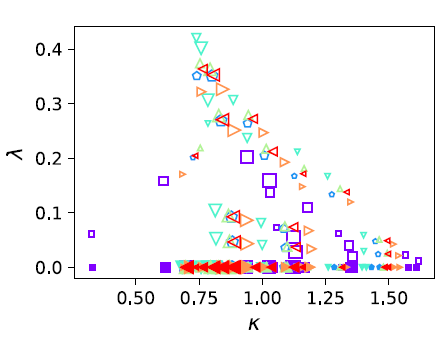
\includegraphics[width=1.4 \columnwidth]{Paper Image.png}
    \caption{This figure has been taken from \citet{2019MNRAS.487..993D}. The x-axis shows the dimensionless energy parameter while the y-axis shows the dimensionless spin parameter. For a more detailed explanation, we refer the readers to \citet{2019MNRAS.487..993D}. Open points indicate
    tangential initial velocities, and filled points denote radial initial velocities. Colors tell the six different density profiles analyzed in the original paper.}
    \label{Paper}
\end{figure*}

\begin{figure*}[ht]
    \centering
    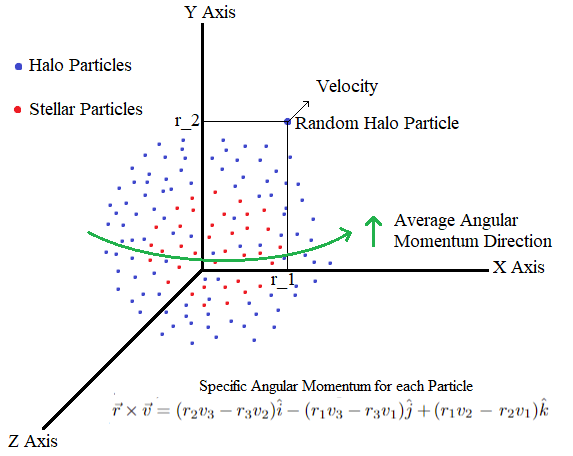
\includegraphics[width=1.4 \columnwidth]{Method Pict.png}
    \caption{This figure shows a general galaxy halo and stellar particle distribution. We also show a random halo particle's velocity and x, y, and z coordinates (Note: z coordinate for the selected particle is 0 in this case). We also plot an example of the direction of the angular momentum of the whole body.}
    \label{Method}
\end{figure*}

\subsection{First Guess at the Results}

As the halo spin correlates with the disk spin, we believe that the angle of ASAM for individual galaxies should be close to the angle of ASAM of galaxies' disks. Estimating the magnitudes of spins of M31 and MW is an area of active research. Thus our simple estimates should be consistent with current literature. For the halo merger remnant, however, multiple factors, such as the angle of collision,  the relative orientation of the halo spins right before the collision, etc., will play an important role. Nonetheless, as the number of halo particles increases post-merger, and the relative velocity plot (for MW and M31) shows zero velocity (but individual velocities decrease in magnitude) after galaxies have merged, we can guess that the halo remnant should have less spin than the sum of individual galaxy spins before the merger. 

%% IMPORTANT! The old "\acknowledgment" command has be depreciated. It was
%% not robust enough to handle our new dual anonymous review requirements and
%% thus been replaced with the acknowledgment environment. If you try to 
%% compile with \acknowledgment you will get an error print to the screen
%% and in the compiled pdf.
%% 
%% Also note that the akcnowlodgment environment does not support long amounts of text. If you have a lot of people and institutions to acknowledge, do not use this command. Instead, create a new \section{Acknowledgments}.


%% For this sample we use BibTeX plus aasjournals.bst to generate the
%% the bibliography. The sample631.bib file was populated from ADS. To
%% get the citations to show in the compiled file do the following:
%%
%% pdflatex sample631.tex
%% bibtext sample631
%% pdflatex sample631.tex
%% pdflatex sample631.tex

\clearpage
\bibliography{sample631}{}
\bibliographystyle{aasjournal}

%% This command is needed to show the entire author+affiliation list when
%% the collaboration and author truncation commands are used.  It has to
%% go at the end of the manuscript.
%\allauthors

%% Include this line if you are using the \added, \replaced, \deleted
%% commands to see a summary list of all changes at the end of the article.
%\listofchanges

\end{document}

% End of file `sample631.tex'.
